\documentclass[12pt]{beamer}
\usetheme{Boadilla}
\usepackage{booktabs}
\usepackage{multirow}
\usepackage{enumitem}
\usepackage{tikz}

\newcommand{\E}{\mathbb{E}}
\usefonttheme{professionalfonts}
\usepackage{pgfplots}
\pgfplotsset{compat=1.18}
\renewcommand{\arraystretch}{1.25}
\usetikzlibrary{trees}
\title[ECON2843]{Lecture 14}
\subtitle{Part 3 Estimation and Hypothesis Test}
\date{}
\usepackage{amsmath,amssymb,mathtools,wasysym}
\begin{document}
	\begin{frame}
		\titlepage
	\end{frame}
	\begin{frame}
		\vspace{1cm}
		\centering
		{\color{blue}\large Hypothesis Test}
	\end{frame}
	
\begin{frame}
	\frametitle{2. Test Statistic}
	
	\begin{itemize}[label={\color{blue}$\blacktriangleright$}]
		\item The test statistic is a sample statistic that we use as a criterion to determine whether or not to reject $H_0$.
		\item It is usually based on an estimator of the population parameter that we are testing.
		\item Bowling example:
		\begin{itemize}[label={\color{blue}$\blacktriangleright$}]
			\item $\bar{X} = 80$, i.e., sample mean bowling score from 10 games.
		\end{itemize}
	\end{itemize}
	
\end{frame}
\begin{frame}
	\frametitle{3. Decision Rule}
	
	\begin{itemize}[label={\color{blue}$\blacktriangleright$}]
		\item In order to make our decision about the hypotheses,we need to know the sampling distribution of the test statistic under $H_0$, called the {\bf null distribution}.
		\item Remember that we always start by assuming $H_0$ is true.
		\item {\color{red}If the observed value of the test statistic is extreme (i.e., very unlikely to occur under the null distribution), then that is evidence against $H_0$.}
	\end{itemize}
	
\end{frame}
\begin{frame}
	\frametitle{Rejection Region}
	
	\begin{itemize}[label={\color{blue}$\blacktriangleright$}]
		\item Whether or not an observed test statistic is extreme is determined by the \textit{rejection region} or \textit{p-value} (more on \textit{p}-values later).
		
		\item The \textbf{rejection region} is a range of values such that, if the test statistic falls within this range, we reject $H_0$.
		
		\item Bowling example:
		\begin{itemize}[label={\color{blue}$\blacktriangleright$}]
			\item The rejection region might be any sample mean less than 120, i.e., $\bar{X} < 120$.
		\end{itemize}
	\end{itemize}
	
\end{frame}
\begin{frame}
	\frametitle{Critical Values}
	
	\begin{itemize}[label={\color{blue}$\blacktriangleright$}]
		\item Related to the rejection region are the {\bf critical values}, which are the values which represent the boundaries of the rejection region.
		
		\item That is, values of the test statistic {\sl more extreme }than the critical values define the rejection region.
		
		\item Bowling example:
		\begin{itemize}[label={\color{blue}$\blacktriangleright$}]
			\item The critical value was $c = 120$ and any sample mean less than $c$ lies in the rejection region.
		\end{itemize}
	\end{itemize}
	
\end{frame}

\begin{frame}
	\frametitle{4. Conclusion}
	
	\begin{itemize}[label={\color{blue}$\blacktriangleright$}]
		\item Final step of the hypothesis test.
		
		\item If the observed test statistic falls in the rejection region, we reject $H_0$ and conclude that $H_1$ is true.
		
		\item If the observed test statistic does not fall in the rejection region, we fail to reject $H_0$ and conclude that $H_0$ is true.
		\item Note that we do not "accept $H_0$".
	\end{itemize}
	
\end{frame}
\begin{frame}
	\frametitle{Type I and Type II Errors}
	
	\begin{table}
		\centering
		\begin{tabular}{cccc}
			\toprule
			&& \multicolumn{2}{c}{Truth} \\
			\cline{3-4}
			&& $H_0$ is true & $H_0$ is false \\
			\midrule
			\multirow{4}{*}{Decision} &\multirow{2}{*}{Reject $H_0$ }  & Type I error &\multirow{2}{*}{Correct decision}  \\
			&& $P(\text{Type I error}) = \alpha$ & \\
			\cline{2-4}
			&Fail to &\multirow{2}{*}{Correct decision}  & Type II error \\
		&reject $H_0$ & &$P(\text{Type II error}) = \beta$ \\
			\bottomrule
		\end{tabular}
	\end{table}
	

	\begin{itemize}[label={\color{blue}$\blacktriangleright$}]
		\item \textbf{Type I error}: Rejecting $H_0$ when it is actually true.
		\item \textbf{Type II error}: Failing to reject $H_0$ when it is actually not true.
	\end{itemize}
	
\end{frame}
\begin{frame}
	\frametitle{Type I and Type II Errors}
	\begin{itemize}[label={\color{blue}$\blacktriangleright$}]
		\item For any hypothesis test, we would like both errors to be small.
		\item However, trying to make one small often causes the other to be large.
		\item Type I error considered more serious than type II error.
		\item $\alpha=P$ (Type I error) is also called the {\bf significance level} of the test.
	\end{itemize}
	
\end{frame}
\begin{frame}
	\frametitle{Type I Error}
	\begin{itemize}[label={\color{blue}$\blacktriangleright$}]
		\item The value of $\alpha$ is usually fixed beforehand and we try to keep it small.
		\item The value of $\alpha$ (together with $H_1$) determines the rejection region.
		\item The smaller the value of $\alpha$, the more sure we can be of our decision if we end up rejecting $H_0$.
	\end{itemize}
	
\end{frame}

\begin{frame}
	\frametitle{Type I Error}
	\begin{itemize}[label={\color{blue}$\blacktriangleright$}]
		\item For the bowling example, the shaded area is equal to $\alpha$.
		\centering
		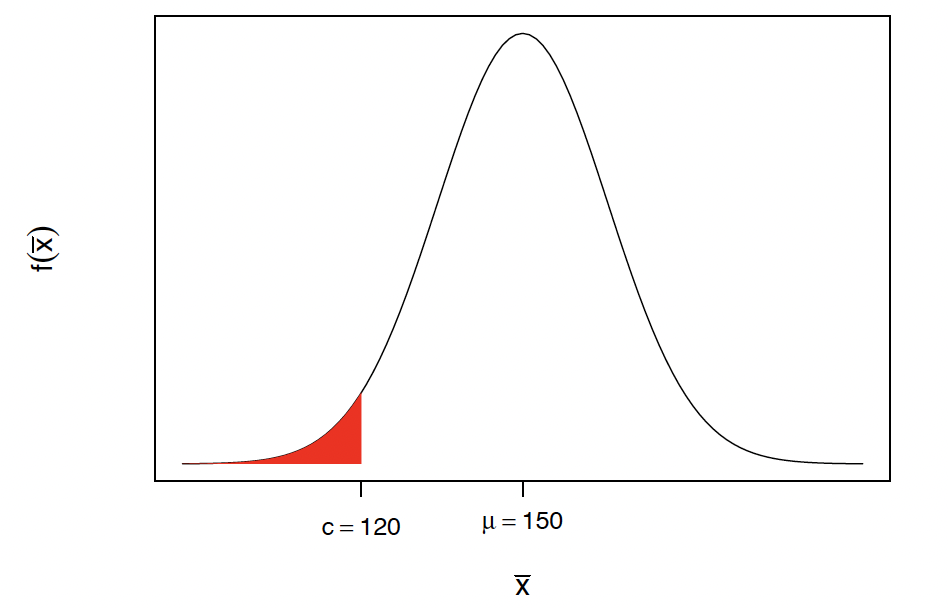
\includegraphics[width=11cm]{type1.png}
	\end{itemize}
	
\end{frame}
\begin{frame}
	\frametitle{Summary}
	
	\begin{enumerate}[label=\textcolor{blue}{\arabic*.}]
		\item Hypotheses:
		\begin{itemize}[label={\color{blue}$\blacktriangleright$}]
			\item Establish $H_0$ and $H_1$.
			\item Assume $H_0$ is true.
		\end{itemize}
		
		\item Test statistic:
		\begin{itemize}[label={\color{blue}$\blacktriangleright$}]
			\item Obtain a sample and calculate a test statistic.
		\end{itemize}
		
		\item Decision rule:
		\begin{itemize}[label={\color{blue}$\blacktriangleright$}]
			\item Determine the rejection region of the null distribution (based on $H_1$ and $\alpha$).
		\end{itemize}
		
		\item Conclusion:
		\begin{itemize}[label={\color{blue}$\blacktriangleright$}]
			\item If the observed test statistic is extreme, i.e., falls in the rejection region, reject $H_0$.
			\item If not, fail to reject $H_0$.
		\end{itemize}
	\end{enumerate}
	
\end{frame}
\begin{frame}
	\frametitle{Hypothesis Test for $\mu$ when $\sigma^2$ is Known}
	
	\begin{itemize}[label={\color{blue}$\blacktriangleright$}]
		\item Hypotheses:
		\begin{align*}
			H_0 &: \mu = \mu_0 \\
			H_1 &: \mu(\neq, <, >)\mu_0
		\end{align*}
		
		\item Test statistic:
		\begin{equation*}
			Z = \frac{\bar{X} - \mu_0}{\frac{\sigma}{\sqrt{n}}}
		\end{equation*}
	\end{itemize}
	
\end{frame}
\begin{frame}
	\frametitle{Hypothesis Test for $\mu$ when $\sigma^2$ is Known}
	
	\begin{itemize}[label={\color{blue}$\blacktriangleright$}]
		\item Decision rule:
		\begin{itemize}[label={\color{blue}$\blacktriangleright$}]
			\item Under $H_0$, $Z$ has a $N(0,1)$ distribution.
			\item At significance level $\alpha$, rejection regions are:
			\begin{itemize}[label={\color{blue}$\blacktriangleright$}]
				\item $Z > z_{\frac{\alpha}{2}}$ or $Z < -z_{\frac{\alpha}{2}}$ $(H_1 : \mu \neq \mu_0)$.
				\item $Z < -z_{\alpha}$ $(H_1 : \mu < \mu_0)$.
				\item $Z > z_{\alpha}$ $(H_1 : \mu > \mu_0)$.
			\end{itemize}
			\item NB: $z_{\alpha}$ is the value which cuts off an area of $\alpha$ in the upper tail of the $N(0,1)$ distribution.
		\end{itemize}
		
		\item Conclusion:
		\begin{itemize}[label={\color{blue}$\blacktriangleright$}]
			\item If $Z$ falls in the rejection region, reject $H_0$, otherwise, fail to reject $H_0$.
		\end{itemize}
	\end{itemize}
	
\end{frame}
\begin{frame}
	\frametitle{Solve the Bowling Example}
	
	\begin{itemize}[label={\color{blue}$\blacktriangleright$}]
		\item Your lecturer claims to have a bowling average of 150 or higher.
		
		\item You play 10 games with him, and he scores an average of 80.
		
		\item Suppose you know that the standard deviation for bowling scores is 50.
		
		\item Given a 5\% significance level ($\alpha = 0.05$), do you reject your lecturer's claim?
	\end{itemize}
	
\end{frame}
\begin{frame}
	\frametitle{1. Hypotheses}
	
	\begin{itemize}[label={\color{blue}$\blacktriangleright$}]
		\item Set up our hypotheses:
		
		\begin{align*}
			H_0 &: \mu = 150 \\
			H_1 &: \mu < 150
		\end{align*}
		
		\item Assume that $H_0$ is true.
		
		\item Let's draw the null distribution.
	\end{itemize}
	
\end{frame}
\begin{frame}
	\frametitle{Null Distribution}

		\centering
		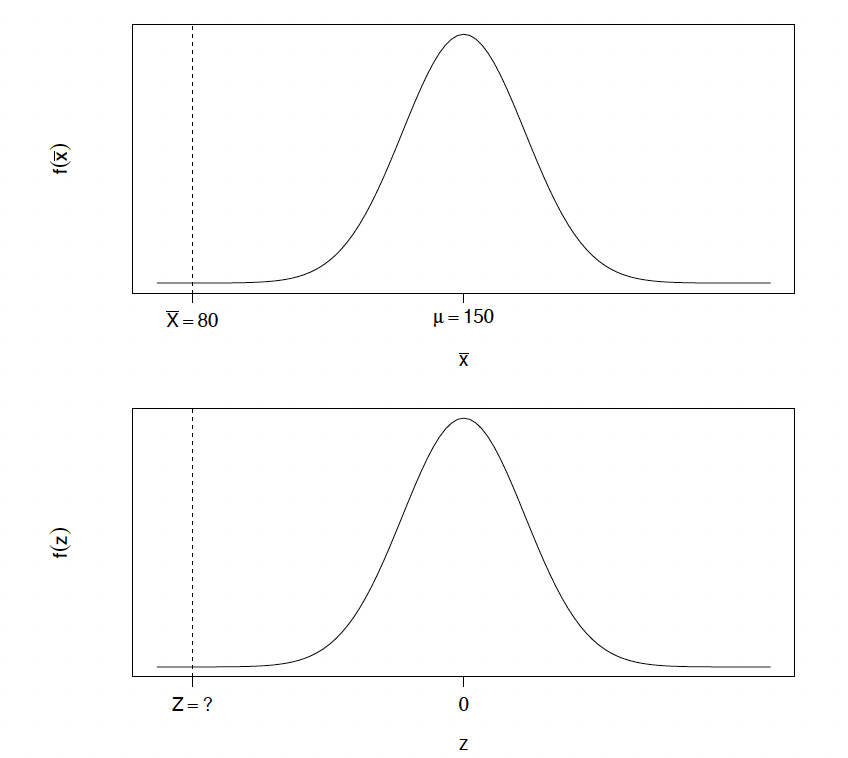
\includegraphics[width=8cm]{null.png}

	
\end{frame}
\begin{frame}
	\frametitle{2. Test Statistic}
	
	\begin{itemize}[label={\color{blue}$\blacktriangleright$}]
		\item Standardize $\bar{X} = 80$:
		
		\begin{equation*}
			Z = \frac{\bar{X} - \mu_0}{\frac{\sigma}{\sqrt{n}}} = \frac{80 - 150}{\frac{50}{\sqrt{10}}} = -4.43
		\end{equation*}
	\end{itemize}
\vspace{0.7cm}
\centering
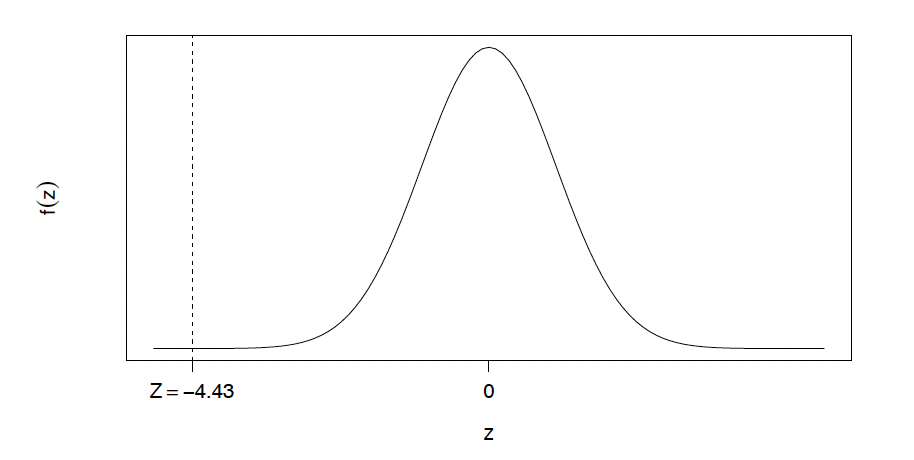
\includegraphics[width=8cm]{test.png}	

\end{frame}
\begin{frame}
	\frametitle{3. Decision Rule}
	
	\begin{itemize}[label={\color{blue}$\blacktriangleright$}]
		\item Rejection region:
		\begin{itemize}[label={\color{blue}$\blacktriangleright$}]
			\item Since $\alpha = 0.05$ and $H_1 : \mu < 150$, find critical value that cuts off 5\% in the left tail of the $N(0,1)$ distribution.
			\item From the $z$-tables, we know $P(Z < -1.645) = 0.05$.
			\item Rejection region is $Z < -z_{0.05} = -1.645$.
		\end{itemize}
	\end{itemize}
\vspace{0.7cm}
\centering
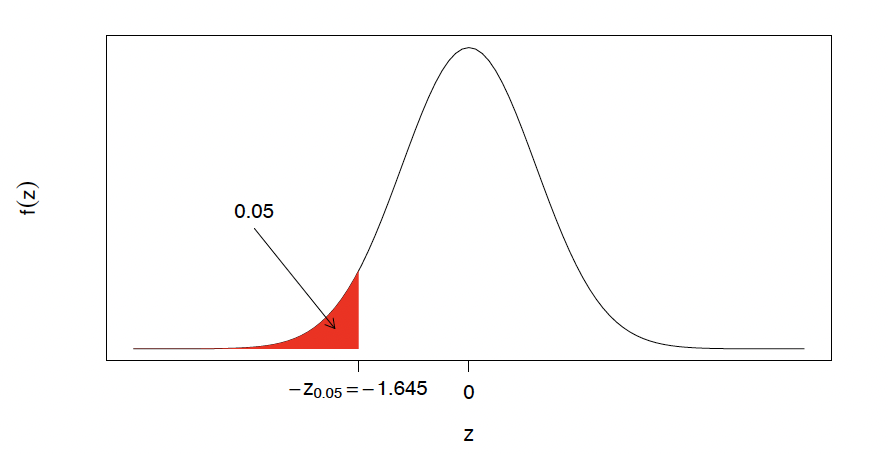
\includegraphics[width=8cm]{test2.png}	

\end{frame}
\begin{frame}
	\frametitle{4. Conclusion}
	
	\begin{itemize}[label={\color{blue}$\blacktriangleright$}]
		\item Since $-4.43 < -1.645$, we reject $H_0$ at the 5\% significance level, and we conclude that my true bowling average is less than $150$.
	\end{itemize}
	\vspace{0.7cm}
	\centering
	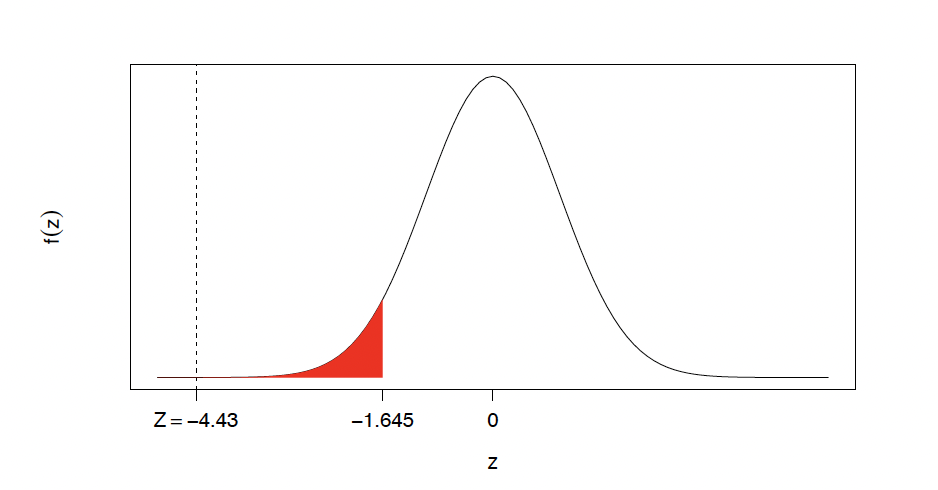
\includegraphics[width=8cm]{test3.png}	
	
\end{frame}
\begin{frame}
	\frametitle{One-Tailed Test}
	
	\begin{itemize}[label={\color{blue}$\blacktriangleright$}]
		\item In a one-tailed test, we only care about one extreme tail of the distribution of the test statistic and the alternative hypothesis usually consists of a ``$>$'' or ``$<$'' sign.
		
		\item For example:
		\begin{itemize}[label={\color{blue}$\blacktriangleright$}]
			\item $H_1 : \mu < 150$.
			\item We only care whether $\mu$ is smaller than 150.
			\item We reject $H_0$ if the test statistic is too small.
		\end{itemize}
	\end{itemize}
	
\end{frame}
\begin{frame}
	\frametitle{Two-Tailed Test}
	
	\begin{itemize}[label={\color{blue}$\blacktriangleright$}]
		\item In a two-tailed test, we care about both extreme tails of the distribution of the test statistic and the alternative hypothesis usually consists of a ``$\neq$'' sign.
		
		\item For example:
		\begin{itemize}[label={\color{blue}$\blacktriangleright$}]
			\item $H_1 : \mu \neq 150$.
			\item Now we care whether $\mu$ is smaller or larger than 150.
			\item We reject $H_0$ if the test statistic is either too small or too large.
		\end{itemize}
	\end{itemize}
	
\end{frame}

\begin{frame}
	\frametitle{Example of a Two-Tailed Test}
	
	\begin{itemize}[label={\color{blue}$\blacktriangleright$}]
		\item Test the following hypothesis:
		
		\vspace{0.5cm}
		
		\begin{align*}
			H_0 &: \mu = 100 \\
			H_1 &: \mu \neq 100
		\end{align*}
		
		\vspace{0.5cm}
		
		when $\bar{X} = 85$, $\sigma = 25$, $n = 15$ and $\alpha = 0.05$.
	\end{itemize}
	
\end{frame}
\begin{frame}
	\frametitle{Null Distribution}
	
	\centering
	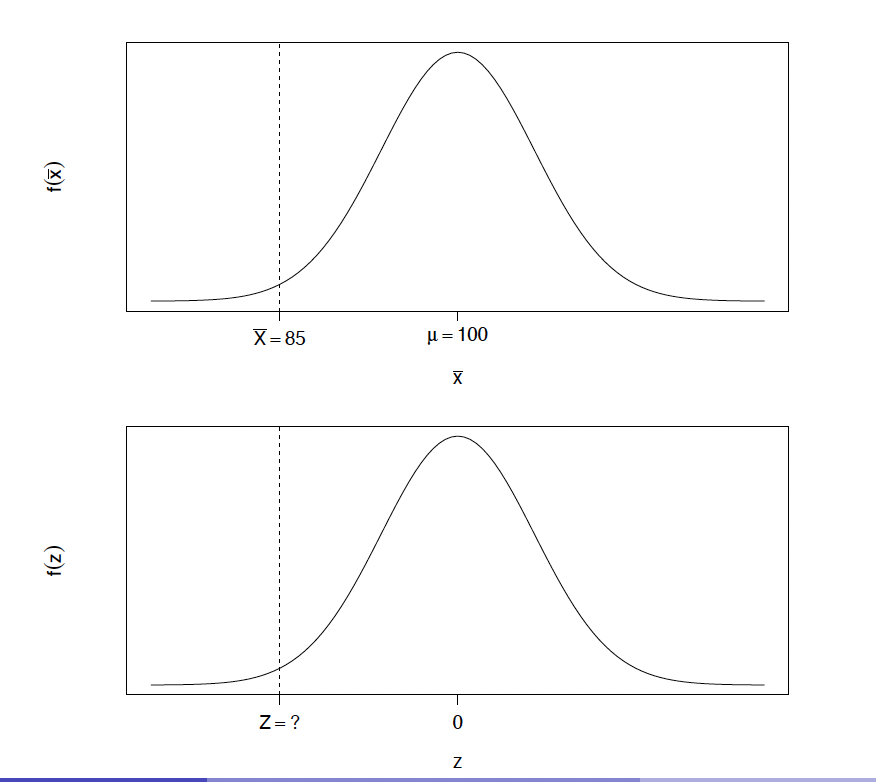
\includegraphics[width=8cm]{null2.png}
	
	
\end{frame}
\begin{frame}
	\frametitle{2. Test Statistic}
	
	\begin{equation*}
		Z = \frac{\bar{X} - \mu_0}{\frac{\sigma}{\sqrt{n}}} = \frac{85 - 100}{\frac{25}{\sqrt{15}}} = -2.32
	\end{equation*}
	\vspace{0.7cm}
	\centering
	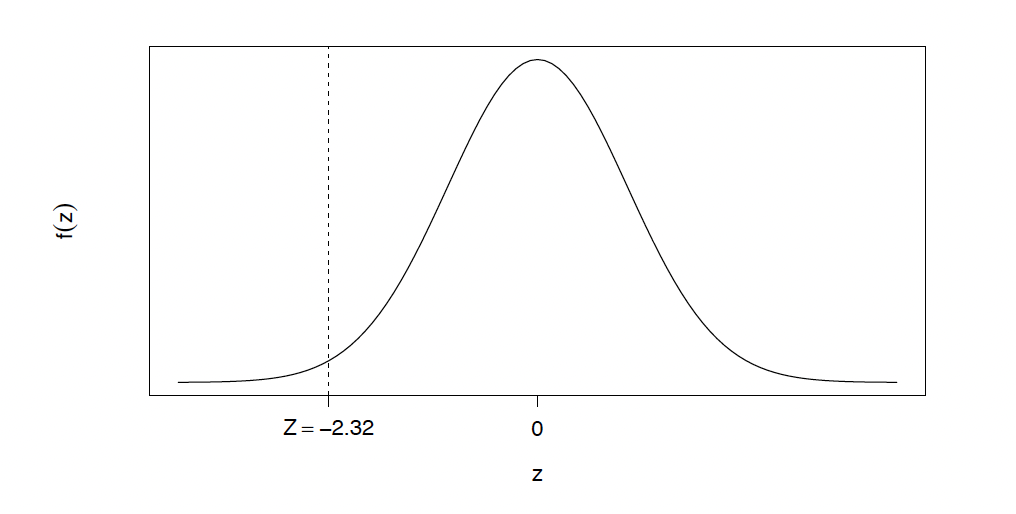
\includegraphics[width=10cm]{test232.png}
\end{frame}
\begin{frame}
	\frametitle{3. Decision Rule}
	
	\begin{itemize}[label={\color{blue}$\blacktriangleright$}]
		\item There are two rejection regions for two-tailed tests!
		
		\item The critical values for the rejection regions are the values that cut off $100 \left(\frac{\alpha}{2}\right) \%$ in each tail of the null distribution. Why?
		
		\item From the $z$-tables, we know that $P(Z > 1.96) = 0.025$.
		
		\item Therefore, by symmetry, the rejection regions are $Z < -1.96$ and $Z > 1.96$.
	\end{itemize}
	
\end{frame}
\begin{frame}
	\frametitle{3. Decision Rule}

	\centering
	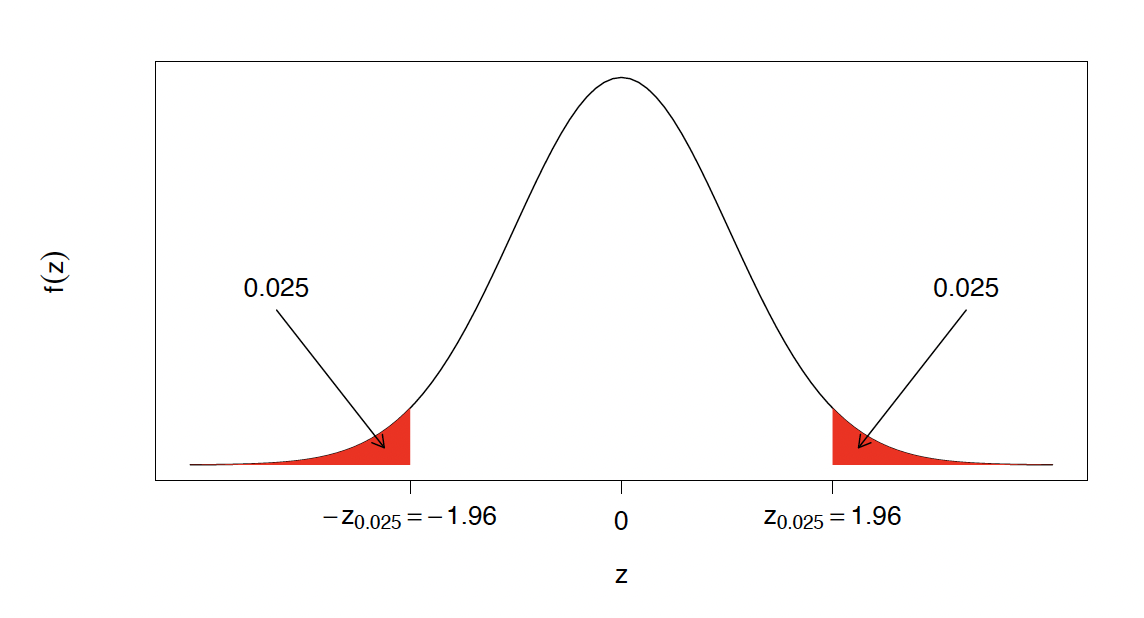
\includegraphics[width=10cm]{decision.png}
\end{frame}
\begin{frame}
	\frametitle{4. Conclusion}
	\begin{itemize}[label={\color{blue}$\blacktriangleright$}]
		\item Since $-2.32<-1.96$, we reject $H_0$.
	\end{itemize}
	\centering
	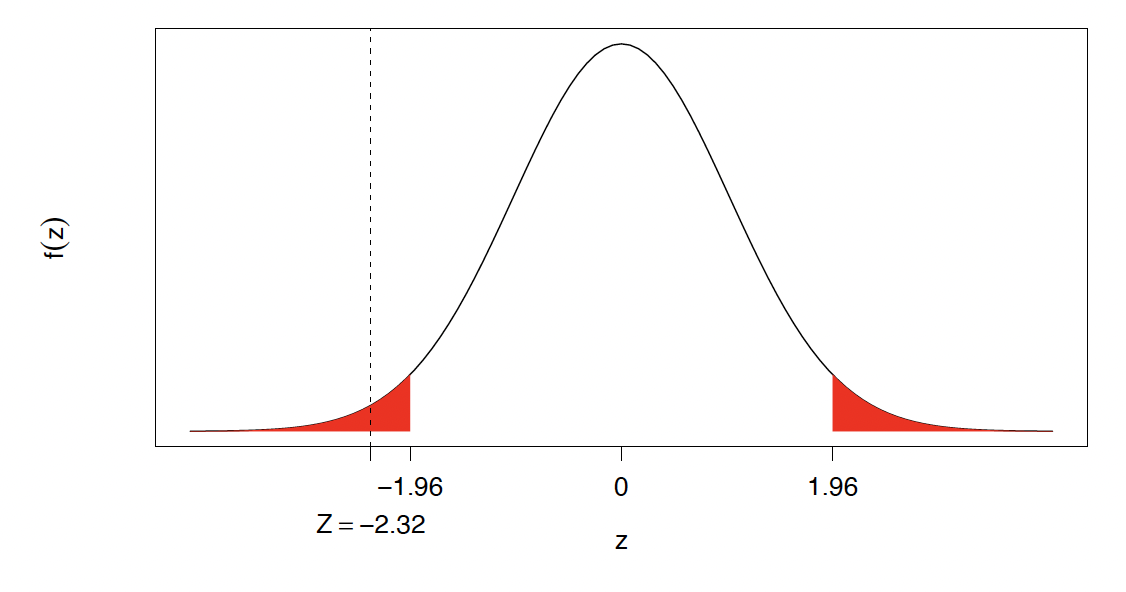
\includegraphics[width=10cm]{conclusion.png}
\end{frame}
\begin{frame}
	\frametitle{Tips on Setting Up Hypotheses}
	
	\begin{itemize}[label={\color{blue}$\blacktriangleright$}]
		\item How we set up our hypotheses is very important.
		
		\item We need to choose $H_0$ and $H_1$ in a way that lets us decide between two distinct situations.
		
		\item The decision then has to help us answer the original question being asked.
	\end{itemize}
	
\end{frame}
\begin{frame}
	\frametitle{Tips on Setting Up Hypotheses}
	
	\begin{itemize}[label={\color{blue}$\blacktriangleright$}]
		\item Remember that $H_0$ usually only includes an ``$=$'' sign.
		
		\item If the question has a claim that includes a ``$<$'', ``$>$'' or ``$\neq$'' sign, set that to be $H_1$.
		
		\item If the question has a claim that includes a ``$\leq$'' or ``$\geq$'' sign, let that claim be represented by $H_0$ and set the opposite claim to be $H_1$.
	\end{itemize}
	
\end{frame}
\begin{frame}
	\frametitle{Example 1}
	
	\begin{itemize}[label={\color{blue}$\blacktriangleright$}]
		\item A school teacher believes they are an excellent teacher and that the average exam score of students in their class is greater than 85. Test the school teacher's claim.
		
		\item Let $\mu$ be the population mean exam score.
	\end{itemize}
	
\end{frame}
\begin{frame}
	\frametitle{Example 1}
	
	\begin{itemize}[label={\color{blue}$\blacktriangleright$}]
		\item The question includes the claim $\mu > 85$. So we should set:
		
		\begin{align*}
			H_0 : \mu &= 85 \\
			H_1 : \mu &> 85
		\end{align*}
		
		\item If we reject $H_0$, we conclude the average exam score is greater than 85 and if we fail to reject $H_0$, we conclude the average exam score is not greater than 85.
	\end{itemize}
	
\end{frame}

\begin{frame}
	\frametitle{Example 2}
	
	\begin{itemize}[label={\color{blue}$\blacktriangleright$}]
		\item A policeman believes that the average speed of motorists on a street that has a speed limit of 40 mph is at least 51 mph. Test the policeman's claim.
		
		\item Let $\mu$ denote the population mean speed.
	\end{itemize}
	
\end{frame}

\begin{frame}
	\frametitle{Example 2}
	
	\begin{itemize}[label={\color{blue}$\blacktriangleright$}]
		\item The question includes the claim $\mu \geq 51$, and the opposite claim is $\mu < 51$. So we should set:
		
		\begin{align*}
			H_0 : \mu &= 51 \\
			H_1 : \mu &< 51
		\end{align*}
		
		\item If we reject $H_0$, we conclude that the mean speed is less than 51 and if we fail to reject $H_0$, we conclude that the mean speed is at least 51.
	\end{itemize}
	
\end{frame}
\begin{frame}
	\frametitle{Example 3}
	
	\begin{itemize}[label={\color{blue}$\blacktriangleright$}]
		\item An office manager believes that the average number of sick days his staff take in a year is at most 13 days. Test the office manager's claim.
		
		\item Let $\mu$ denote the population mean number of sick days taken.
	\end{itemize}
	
\end{frame}
\begin{frame}
	\frametitle{Example 3}
	
	\begin{itemize}[label={\color{blue}$\blacktriangleright$}]
		\item The question includes the claim $\mu \leq 13$, and the opposite claim is $\mu > 13$. So we should set:
		
		\begin{align*}
			H_0 : \mu &= 13 \\
			H_1 : \mu &> 13
		\end{align*}
		
		\item If we reject $H_0$, we conclude that $\mu$ is greater than 13 and if we fail to reject $H_0$, we conclude that $\mu$ is at most 13.
	\end{itemize}
	
\end{frame}

\begin{frame}
	\frametitle{$p$-value}
	
	\begin{itemize}[label={\color{blue}$\blacktriangleright$}]
		\item There are two ways of conducting hypothesis tests:
		\begin{enumerate}[label=\arabic*.]
			\item Using rejection regions.
			\item Using $p$-values.
		\end{enumerate}
		
		\item A \textbf{$\boldsymbol{p}$-value} is the probability of observing a test statistic even more extreme than the one calculated from your sample, assuming that $H_0$ is true.
	\end{itemize}
	
\end{frame}
\begin{frame}
	\frametitle{Example}
	
	\begin{itemize}[label={\color{blue}$\blacktriangleright$}]
		\item Suppose we are testing the following hypotheses:
		
		\begin{align*}
			H_0 : \mu &= 140 \\
			H_1 : \mu &> 140
		\end{align*}
		
		\item Further, suppose our standardized $Z$-statistic turns out to be $Z = 1.10$.
		
		\item What is the $p$-value?
	\end{itemize}
	
\end{frame}

\begin{frame}
	\frametitle{Example}
	
	\begin{itemize}[label={\color{blue}$\blacktriangleright$}]
		\item The $p$-value is the probability of observing something more extreme than $Z = 1.10$.
		
		\item Because of our one-tailed alternative hypothesis, more extreme means greater than 1.10.
		
		\item The $p$-value:
		
		\begin{align*}
			P(Z > 1.10) &= 1 - P(Z < 1.10) \\
			&= 1 - 0.8643 \\
			&= 0.1357
		\end{align*}
	\end{itemize}
	
\end{frame}
\end{document}